\documentclass[12pt,letterpaper,noanswers]{exam}
%\usepackage{color}
\usepackage[usenames,dvipsnames,svgnames,table]{xcolor}
\usepackage[margin=0.9in]{geometry}
\renewcommand{\familydefault}{\sfdefault}
\usepackage{multicol}
\pagestyle{head}
\usepackage{hyperref}
\usepackage[numbered,autolinebreaks,useliterate]{mcode}
\newcommand{\mb}[1]{\underline{#1}}

\header{AM 22b Problem Set 08}{}{Due Thurs Apr 8 at 6pm EDT}
\runningheadrule
\headrule
\usepackage{diagbox}
\usepackage{graphicx} % more modern
%\usepackage{subfigure} 
\usepackage{amsmath} 
\usepackage{amssymb} 
%\usepackage{gensymb} 
%\usepackage{natbib}
\usepackage{hyperref}
%\usepackage{enumitem}
%\setlength{\parindent}{0pt}
%\usepackage{setspace}
%\pagestyle{empty}  
%\newcommand{\Sc}[0]{
%{\color{BlueViolet}\S}
%}
\usepackage{tcolorbox}

\begin{document}
 \pdfpageheight 11in 
  \pdfpagewidth 8.5in

\begin{questions}
\question Log in to WeBWorK and complete the problems assigned there under pset08.  \emph{For the last two questions, see \S 19.2 for the area element of a cylindrical surface in cylindrical coordinates and of a spherical surface in spherical coordinates.}


\question A common model for laminar flow of an incompressible fluid through a pipe, where the flow is driven by pressure, is called Poiseuille flow.  



During Poiseuille flow, the speed of liquid through a pipe with circular cross-section is proportional to \[a^2-r^2\] where $a$ is the radius of the pipe and $r$ is the distance from the center of the pipe.  

\begin{parts}
\item Water is flowing down a cylindrical pipe of radius $6$ mm. Up to the unknown constant of proportionality, find the flux through a circular cross-section of the pipe.  Orient the surface so that the flux is positive.



\begin{solution}
We want to find the flux through the circular cross section.  It is oriented so that the flux is positive.  I'll let the pipe run along the $y$-axis, so that the velocity vectors for the water point in the positive $\vec j$ direction.  We have $\vec v = k(a^2-r^2)\vec j$ where $k$ is a constant of proportionality (not given in this problem).  Since the velocity is in distance per time and $a$, $r$ are in distance, the units of $k$ must be $1/(\text{distance}\cdot\text{time})$.  The cross section is a flat piece of the plane and its area vector is $\vec A = \pi a^2 \vec j$, since this cross section is perpendicular to the pipe.

A piece of this cross section has area vector $d\vec A = r drd\theta \vec j$.  The flux is
\begin{align*}
\text{Flux } &= \int_S \vec v \cdot d\vec A \\
&= \int_0^{2\pi}\int_0^a k(a^2-r^2) r\ dr\ d\theta \\
&= k\int_0^{2\pi} \left. \frac{1}{2}a^2r^2 - \frac{1}{4}r^4 \right\vert_0^a d\theta \\
&= \frac{k}{2} \int_0^{2\pi} a^4 - \frac{1}{2}a^4\ d\theta \\
&= \frac{k}{2}\frac{a^4}{2}2\pi \\
&= \frac{1}{2}ka^4\pi.
\end{align*}
This has units of  $1/(\text{distance}\cdot\text{time})$$\cdot$distance$^4$ so volume per time, as expected!

For $a = 6$ mm, we have $\frac{1}{2}k(6)^4 \pi$.
\end{solution}

\item Assume a $3$ mm pipe has the same constant of proportionality as the $6$mm pipe above.  How many $3$ mm pipes would be needed to produce the same flux as one $6$ mm pipe?
\begin{solution}
The flux through a pipe of radius $a$ is $\frac{1}{2}ka^4\pi$, so if the radius is $b = a/2$ we have $\frac{1}{2}k b^4\pi = \frac{1}{2}ka^4\pi/16$.  We need $16$ pipes of radius $3$ mm to match the flow rate through one pipe of radius $6$ mm. 
\end{solution}
\item Use Matlab to plot the velocity vectors of the water for a cross-section of a $6$ mm pipe and a cross-section of a $3$-mm pipe (show the velocity for the full diameter of the pipe and use the same length scale for all vectors).  \emph{You can use the Matlab code below for the 6 mm pipe, or can write your own.}

If you use the \texttt{quiver} command as part of your plotting, use \texttt{doc quiver} to learn about the command and briefly summarize what the command does as part of your answer.

\begin{lstlisting}
hold off
% Plot the velocity vectors for the 6mm pipe.
aval = 6;
numbervectors = 11;
% find coordinates of the z-points:
zval = linspace(-aval,aval,numbervectors); 
% all x-values are 0:
xval = zeros(size(zval));
% horizontal velocity:
xvec = aval^2-zval.^2; 
% vertical velocity is zero:
zvec = zeros(size(zval)); 
% plot vectors (xvec, zvec) at points (xval, zval).:
quiver(xval, zval, xvec, zvec,'b','autoscale','off') 
hold on
% plot the points on the bounding curve showing the lengths of the vectors.
plot(xvec,zval,'b')
\end{lstlisting}
% % Make the same plot for the 3mm pipe.
% aval = 3;
% zval = linspace(-aval,aval,numbervectors);
% xval = zeros(size(zval));
% xvec = aval^2-zval.^2;
% zvec = zeros(size(zval));
% quiver(xval, zval, xvec, zvec,'r','autoscale','off')
% plot(xvec,zval,'r')
% axis equal
% set(gca,'fontsize',14)
% xlabel('speed of fluid')
% ylabel('position along pipe diameter')

\end{parts}

Three video links of fluid flow:
\begin{itemize}
    \item {\color{blue}\href{https://www.youtube.com/watch?v=rknHorDj3Vk}{Link1: laminar pipe flow with corrugated edge}}
    \item {\color{blue}\href{https://www.youtube.com/embed/JO5U3aZlMzM?start=75&end=120&autoplay=1}{Link2: laminar and turbulent flows}}
    \item Not Poiseuille flow, but an interesting demo of laminar Couette flow.  This is fluid motion that is driven by drag on the walls instead of by pressure. \href{https://www.youtube.com/watch?v=nvmtPsBlCAs}{\color{blue} Link3: reversible laminar flow demo - watch at double speed.}
\end{itemize}

\quad  





\question  Let $\vec F = yz\vec i + xy\vec j + xy\vec k$ and let $S$ be the part of the graph of $z = \cos x + \sin 2y$ whose projection into the $xy$-plane, $R$, is the triangle with vertices $(0,0)$, $(0,5)$, $(5,0)$.

\emph{The surface is shown over the square region $0\leq x\leq 5, 0\leq y\leq 5$.  The blue vectors are proportional to the area vectors of the vector field while the red vectors are proportional to the vector field itself.}

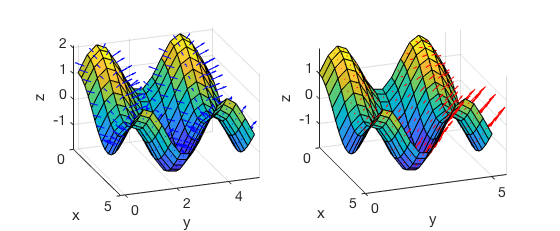
\includegraphics[width=\linewidth]{img/pset11p1-18.png}

\begin{lstlisting}
% The plot is for a square region in the xy-plane even though the problem
% is for a triangle.
% Plot the surface in each subplot:
for k = 1:2
    subplot(1,2,k)
    hold off
    % Choose x values between 0 and 5.  Make 10 of them.
    xint = linspace(0,5,15);
    % Use the same values of y.
    yint = xint;
    % Make a grid of x and y values at which we want to plot.
    % This is a grid of corners of parallelograms.
    [xv, yv] = meshgrid(xint, yint);
    % z-values on the surface:
    zv = cos(xv)+sin(2*yv);
    % Make a grid of the center points of the parallelograms 
    % (by averaging pairs of coordinates.)
    xvc = (xv(1:end-1,1:end-1)+xv(2:end,2:end))/2;
    yvc = (yv(1:end-1,1:end-1)+yv(2:end,2:end))/2;
    zvc = (zv(1:end-1,1:end-1)+zv(2:end,2:end))/2;
    hold off
    % plot the surface parallelograms:
    surf(xv, yv, zv)%,'facealpha',0.7)
    hold on
    view(70,21)
end
\end{lstlisting}
\begin{lstlisting}
% Vectors aligned with area vectors are drawn on the surface in the first 
% subplot.
subplot(1,2,1)
% create <-f_x, -f_y, 1> to draw vectors proportional to the area vector
% at the corner of each parallelogram:
xareavec = sin(xvc);
yareavec = -2*cos(2*yvc);
zareavec = ones(size(xvc));
quiver3(xvc, yvc, zvc, xareavec, yareavec, zareavec,'b')
% Vectors aligned with the vector field are drawn on the surface in the
% second subplot.
subplot(1,2,2)
F1 = yvc.*zvc;
F2 = xvc.*yvc;
F3 = xvc.*yvc;
quiver3(xvc, yvc, zvc, F1, F2, F3,'r','autoscalefactor',2)
for k=1:2
    subplot(1,2,k)
    axis equal
    xlabel('x'); ylabel('y'); zlabel('z');
    set(gca, 'fontsize',14)
end
\end{lstlisting}
\begin{parts}
\part Construct a normal vector, $\underline n$, to the point on the surface graph of $f(x,y) = \cos x + \sin 2y$ associated with the input $(a,b)$.
\begin{solution}
$\langle -f_x, -f_y, 1\rangle$ is normal to the surface $z = f(x,y)$ at the point $(x,y,z)$, so $\langle \sin x, -2\cos 2y, 1\rangle$ is a normal vector.
\end{solution}
\part Based on the code above, identify the following line numbers:
\begin{itemize}
    \item Identify the line number where the $z$-value of the surface coordinates is determined.
    \item Identify the line numbers where the components of the normal vectors to the surface are defined.
    \item Identify the line numbers where the vector field components are defined.
    \item Identify the line numbers where the vector fields are plotted.
\end{itemize}
Use \texttt{doc quiver3} to learn about the \texttt{quiver3} command.  Briefly summarize what the command does.
\begin{solution}
The z-value of the surface coordinates is found in line 15: $z = \cos(x) + \sin(2*y)$.

The normal vectors to the surface are defined in lines 6-8 (they components are called xareavec, yareavec, zareavec).

The vector field is defined in lines 13 to 15.

The vector field is plotted in line 16.  The area vectors are plotted in line 9.

The command \texttt{quiver3} takes in points and vectors, and plots the vectors at the points.
\end{solution}
\part Set up an interated integral to compute the flux of $\underline F$ through $S$.  Do \textbf{not} integrate.

Repeat of the problem info:
$\underline F = yz\underline i + xy\underline j + xy\underline k$.  $S$ is the part of the graph of $z = \cos x + \sin 2y$ whose projection into the $xy$-plane, $R$, is the triangle with vertices $(0,0)$, $(0,5)$, $(5,0)$.
\end{parts}



\question
Let $W$ be the solid region bounded below by $z = x^2+y^2$ and bounded above by $z = \sqrt{6-x^2-y^2}$.  Let $S_1$ be the paraboloid forming the lower surface of $W$, oriented upward.  % Let $S_2$ be the spherical cap forming the upper surface of $W$, also oriented upward.
% \begin{parts}
% \item 
Use a flux integral to find the flux of $\underline F =\langle x, y, z\rangle$ upward through $S_1$.
%\part Use a flux integral to find the flux of $\vec F = x\vec i + y\vec j + z\vec k$ upward through $S_2$.
%\end{parts}


\question According to Coulomb's Law, the electric field produced by a point charge $q$ placed at the origin is $\displaystyle \underline F = \frac{q}{\Vert \underline r\Vert^2}\frac{\underline r}{\Vert \underline r\Vert}$.  This vector field is undefined at the origin.

 Show that the flux out of a sphere, $S$, centered at the origin and oriented-outward, is $4\pi q$.
 
 
 

\item An acoustic Doppler current profiler (ADCP) is attached to a boat that traverses the Charles River, measuring the velocity profile of the water, $\mb F(x,y,z) = \langle F_1, F_2, 0\rangle$ in meters per second, at points beneath the path of the boat.  \emph{The $z$-component of the water velocity may be nonzero, but it is not contributing to the flux downstream, so we will set it to zero for these calculations.} 

The path of the boat, $C$, is given by $\mb r(t) = \langle x(t), y(t), 0\rangle$ for $0\leq t \leq 600$ seconds (10 minutes).  It's velocity is $\langle u(t), v(t), 0 \rangle$ where $u(t) = \dot x$ and $v(t) = \dot y$ (recall $\dot x$ denotes $\frac{dx}{dt}$), with $u,v$ measured in meters per second.  Assume the boat is oriented as in the image below.  Downstream is on the starboard side of the boat.

Let the profile of the bottom of the river be given by $z = f(x,y)$.  \emph{Note that points on the river bottom have $z < 0$.}

Let $S$ be the (imaginary) surface reaching vertically from the path of the boat to the bottom of the river.  It is shown in light blue in the image below.  Points on this surface are of the form $(x(t), y(t), z)$ where $0\leq t\leq 600$ seconds and $f(x(t),y(t)) \leq z \leq 0$.  

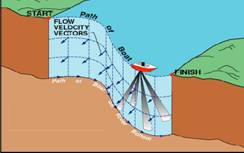
\includegraphics{img/S20pset08USGS.png}

Image from \url{https://hydroacoustics.usgs.gov/movingboat/index.shtml} Accessed April 2020.

\begin{parts}
\part Set up an integral for the length of the path $C$.  Write it in terms of $u$ and $v$.
\begin{solution}
$\int_C ds = \int_0^{600}\sqrt{u^2+v^2}dt$
\end{solution}

\part Each point along the path has an associated river depth.  Use this to set up an iterated double integral for the area of the surface $S$. 

\emph{Think of this as a lot like finding the area of a fence.  You have a curve telling you the shape of the fence and you know the height of the fence at each point along the curve.}

\emph{Write the integral in the form $\displaystyle\int_0^{600} \int_?^? ? \ dz\ dt$.}

\begin{solution}
We have a height at each point along $C$, so the area is as follows
$\text{area } = \int_C h(s) ds = \int_C \int_{f(x(t),y(t))}^0 dz ds = \int_0^{600}\int_{f(x(t),y(t))}^0 \sqrt{u^2+v^2}\ dz\ dt$
\end{solution}


\item Consider a small piece of the surface with sides given by the vectors $\langle 0, 0, \Delta z\rangle$ and $\langle \Delta x, \Delta y, 0\rangle$. 
\begin{itemize}
\itemsep0em
    \item Use linear approximation to express $\Delta x$ and $\Delta y$ in terms of $\Delta t$.
    \item Find $\Delta\underline S$ for this piece of the surface. \emph{$\Delta \underline S$ is a vector that points normal to the piece of surface, and $\Vert \Delta \underline S\Vert$ is equal to the area of the piece.}
    \item Choose $\Delta \underline S$ so that the normal direction is oriented downstream (rather than upstream).
\end{itemize}
\begin{solution}
$\Delta x \approx \frac{dx}{dt}\Delta t = u\Delta t$ and $\Delta y \approx v\Delta t$.

The sides of the parallelogram are $\underline w_1 = \langle u, v, 0\rangle \Delta t$ and $\underline w_2 \langle 0,0,1\rangle\Delta z$.

$\Delta \underline S = \underline w_1 \times \underline w_2$ or $\underline w_2\times\underline w_1$.  We know that $\underline w_1$ points in the direction of the motion of the boat and (looking from above) downstream is clockwise from that direction.  Using the right hand rule so that the cross product points downstream, I find $\Delta \underline S = \underline w_1 \times \underline w_2$.

This is $\Delta\underline S = \underline w_1 \times \underline w_2 = \left\vert \begin{array}{c c c} \underline i & \underline j & \underline k \\
u\Delta t & v\Delta t & 0 \\
0 & 0 & \Delta z\end{array} \right\vert = v\Delta t\Delta z\underline i- u\Delta t\Delta z \underline j = (v\underline i -u\underline j)\Delta t\Delta z$
\end{solution}

\part Set up an iterated double integral for the flux of $\mb F$ across the surface $S$ in terms of $F_1, F_2, u, v$.

Approximating this integral using measured estimates of the boat velocity, the river velocity, and the profile of the bottom of the river, would give you an estimate of the volume per second of water flowing downstream in the river.

\emph{Your integral will be of the form $\displaystyle\int_0^{600} \int_?^? ? \ dz\ dt$.}

\begin{solution}
$\underline F\cdot \Delta \underline S = (F_1 v - F_2 u)\Delta z \Delta t$.
$\int_S \underline F\cdot d\underline S = \int_0^{600}\int_{f(x(t),y(t))}^0 (F_1 v - F_2 u)\ dz\ dt$
\end{solution}

\part Show that your integrand can be written in terms of $\mb r'(t) \times \mb F$.  \emph{You will need to take a magnitude or use a dot product as your integrand is a scalar and this cross product is a vector.}



\begin{solution}
$\underline r'(t) \times \underline F = \left\vert\begin{array}{c c c} \underline i & \underline j & \underline k \\
u & v & 0 \\
F_1 & F_2 & 0 \end{array}\right\vert = 0\underline i - 0\underline j + (uF_2 - vF_1)\underline k$.

If I assume the flux through each box $\Delta \underline S$ is positive (that there is flow downstream through each box) then $\int_S \underline F\cdot d\underline S = \int_0^{600}\int_{f(x(t),y(t))}^0 (F_1 v - F_2 u)\ dz\ dt = \int_0^{600}\int_{f(x(t),y(t))}^0 \Vert \underline r'(t) \times \underline F\Vert \ dz\ dt$.

If I do not make that assumption, then $\int_S \underline F\cdot d\underline S = \int_0^{600}\int_{f(x(t),y(t))}^0 (F_1 v - F_2 u)\ dz\ dt = \int_0^{600}\int_{f(x(t),y(t))}^0 -(\underline r'(t) \times \underline F)\cdot \underline k \ dz\ dt$

\end{solution}
\end{parts}

Credit to Jory Hecht at the USGS for supplying information about the methods used in the problem above. 
 
% \emph{The area element for a patch of spherical surface is $a^2\sin\phi\ d\phi\ d\theta$ where $a$ is the radius of the sphere.}


% \emph{The area vectors for parallelogram patches of the surface are shown in blue.  The vectors of the vector field are shown in red.}

% 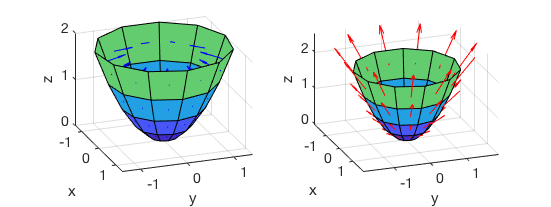
\includegraphics[width=0.4\linewidth]{img/pset11p2-18.png}
% %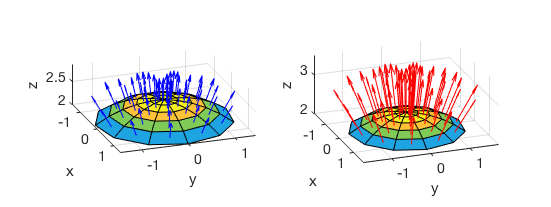
\includegraphics[width=0.4\linewidth]{img/pset11p3-18.png}

% \begin{solution}
% $S_1$: on the paraboloid, $\displaystyle\langle -f_x, -f_y, 1\rangle = \langle -2x, -2y, 1\rangle.$  

% $\displaystyle\int_S \vec F\cdot d\vec A = \int_R \langle x,y,z\rangle \cdot \langle -2x, -2y, 1\rangle dA$ where $R$ is the disk in the $xy$-plane below our surface.  Simplifying, the flux is $\displaystyle\int_R -2x^2-2y^2+z dA = \int_R -2x^2-2y^2+(x^2+y^2) dA =\int_R -r^2 dA$.

% The radius of the disk $R$ is set by the intersection of $z = r^2$ and $z^2 +r^2 = 6$, the two bounding surfaces.  We have $r^4 + r^2 = 6$ so $(r^2)^2+r^2 - 6 = 0$.  $(r^2+3)(r^2-2) = 0$.  $r^2 = -3$ or $r^2= 2$.  Since $r^2 \geq 0$, we have $r^2 = 2 \Rightarrow r = \sqrt{2}$.

% Setting up the integral, $\displaystyle\int_R -r^2\ dA = \int_0^{2\pi}\int_0^{\sqrt{2}} -r^2\ rdrd\theta = \int_0^{2\pi}d\theta\int_0^{\sqrt{2}}-r^3dr = \left.-(2\pi)\frac{r^4}{4}\right\vert_0^{\sqrt{2}} = -2\pi$.

% $S_2$: on the spherical cap (of radius $\sqrt{6})$, the normal vector at a point $(x,y,z)$ is $\vec n = \langle x, y,z\rangle$ and the unit normal vector is $\hat n = \frac{1}{\sqrt{6}}\langle x,y,z\rangle.$  The vector field is $\vec F = \langle x,y,z\rangle$, so $\displaystyle\vec F\cdot \hat n = \frac{1}{\sqrt{6}}(x^2+y^2+z^2) = \frac{\sqrt{6}^2}{\sqrt{6}} = \sqrt{6}.$  The flux integral $\displaystyle\int_{S_2} \vec F\cdot d\vec A = \int_{S_2}\vec F\cdot \hat n\ dS = \int_{S_2} \sqrt{6} dS = \sqrt{6}\text{ Area}(S_2).$  Finding the area of $S_2$ is nontrivial because it isn't an easy piece of sphere.  That surface area will be $\displaystyle\int_0^{2\pi}\int_0^{\phi_0} (\sqrt{6})^2\sin\phi\ d\phi d\theta = -12\pi(\cos\phi_0 - 1)$ (summing the area of small patches of surface).  The flux will be $\displaystyle12\sqrt{6}\pi(1-\cos\phi_0)$.  

% What is $\cos\phi_0$?  $\phi_0$ is the angle between the $z$-axis and the radial line connecting the origin to the circle of intersection.  We know the length of the radial line is $\sqrt{6}$ and we know that the $r$-value associated with the intersection is $\sqrt{2}$.  The $z$-value associated with the intersection can be found by the Pythagorean theorem: $\sqrt{6-2} = \sqrt{4} = 2$.  So $\displaystyle\cos\phi_0 = \frac{2}{\sqrt{6}} = \frac{\sqrt{6}}{3}$.

% The flux is $\displaystyle12\sqrt{6}\pi\left(1-\frac{\sqrt{6}}{3}\right) = 12\sqrt{6}\pi - 24\pi$.
% \end{solution}

% \item Use the divergence theorem to find the flux of $\vec F$ outward through $\partial W$, the boundary of $W$.

% 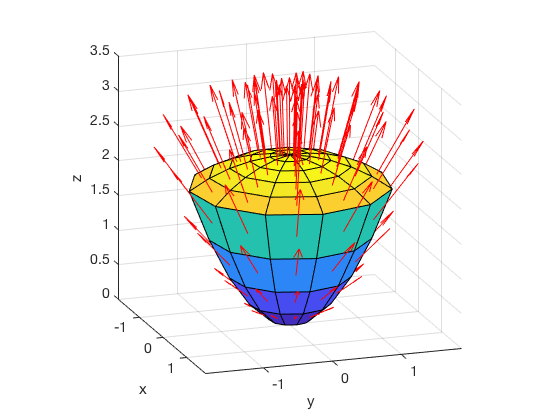
\includegraphics[width=0.4\linewidth]{img/pset11p4-18.png}
% \begin{solution}
% The divergence theorem says $\displaystyle\int_W \text{div }\vec F\ dV = \int_{\partial W} \vec F\cdot d\vec A$.  The divergence of $\vec F$ is $M_x + N_y + P_z$ where $M = x, N=y, P=z$, so div $\vec F = 3$.

% \begin{align*}
%     \int_W \text{div }\vec F\ dV =& \int_0^{2\pi}\int_0^{\sqrt{2}}\int_{r^2}^{\sqrt{6-r^2}}3rdzdrd\theta \\
%     =& \int_0^{2\pi}d\theta\int_0^{\sqrt{2}}\int_{r^2}^{\sqrt{6-r^2}}3rdzdr \\
%     =& 2\pi \int_0^{\sqrt{2}} 3r\left(\sqrt{6-r^2} - r^2\right)dr \\
%     =& \left.2\pi \left(-(6-r^2)^{3/2} - \frac{3}{4}r^4\right) \right\vert_0^{\sqrt{2}} \\
%     =& 2\pi \left(-(6-(\sqrt{2})^2)^{3/2} - \frac{3}{4}\sqrt{2}^4\right) - 2\pi \left(-(6-0^2)^{3/2} - \frac{3}{4}0^4\right) \\
%     =& 2\pi \left(-(4)^{3/2} - 3\right) + 2\pi(6)^{3/2} \\
%     =& -2\pi \left(8 + 3\right) + 12\pi(6)^{1/2}\\
%      =& -22\pi + 12\sqrt{6}\pi
% \end{align*}
% I used $\displaystyle \frac{d}{dr}(6-r^2)^{3/2} = \frac{3}{2}(-2r)(6-r^2)^{1/2} = -3r(6-r^2)^{3/2}$ to get the constants right above.
% \end{solution}

% \item Determine (without integration) the flux through either $S_1$ or $S_2$, with upwards orientation (whichever you didn't find in part (a)).
% \begin{solution}
% $\partial W = S_2 - S_1$ so $\displaystyle\int_{\partial W}\vec F\cdot d\vec A = \int_{S_2} \vec F\cdot d\vec A - \int_{S_1}\vec F\cdot d\vec A$.  I can rearrange:

% $\displaystyle\int_{S_2} \vec F\cdot d\vec A = \int_{\partial W}\vec F\cdot d\vec A + \int_{S_1}\vec F\cdot d\vec A = \left(-22\pi +12\sqrt{6}\pi \right)- 2\pi = -24\pi + 12\sqrt{6}\pi$.

% $\displaystyle\int_{S_1}\vec F\cdot d\vec A = \int_{S_2} \vec F\cdot d\vec A - \int_{\partial W}\vec F\cdot d\vec A = \left(-24\pi + 12\sqrt{6}\pi\right) - (-22\pi+12\sqrt{6}\pi) = -2\pi.$

% Wow, that all actually did work out.  $\partial W = S_2 - S_1$ so

% $\displaystyle\int_{\partial W}\vec F\cdot d\vec A = \int_{S_2} \vec F\cdot d\vec A - \int_{S_1}\vec F\cdot d\vec A$ becomes 

% $-22\pi +12\sqrt{6}\pi = (-24\pi + 12\sqrt{6}\pi)-(-2\pi).$

% \end{solution}
% \end{parts}

% \question 
% \begin{parts}
% \item Let $W$ be a solid region of volume $V$ surrounded by a closed surface $S$, oriented outward.  Show that $\displaystyle \frac{1}{3}\int_S \vec r\cdot d\vec A = V$.  Here the vector field is $\vec r = x\vec i + y\vec j + z\vec k$.
% \begin{solution}
% For this vector field, $\text{div }\vec F = 1 + 1 + 1 = 3$, so we have \[\frac{1}{3}\int_S\vec r\cdot d\vec A = \frac{1}{3}\int_W 3\ dV = \int_W \ dV = V.\]
% \end{solution}
% \item Suppose $\text{div }\vec F = x^2+y^2+3$.  Find a surface, $S$ such that $\int_S\vec F\cdot d\vec A$ is negative (for any vector field where $\text{div }\vec F = x^2+y^2+3$), or explain why no such surface exists.
% \begin{solution}
% By the divergence theorem,
% \[\int_{\partial W} \vec F \cdot d\vec A = \int_W \text{div }\vec F\ dV = \int_W (x^2+y^2+3)\ dV,\] so the flux outward through a closed surface will always be positive.  Let $S$ be a closed surface oriented inward.  Now the flux through the surface will be negative (since the flux will be the negative of the flux outward through that surface).
% \end{solution}
% \end{parts}

% \question According to Coulomb's Law, the electric field produced by a point charge $q$ placed at the origin is $\displaystyle \vec F = \frac{q}{\Vert \vec r\Vert^2}\frac{\vec r}{\Vert \vec r\Vert}$.  This vector field is undefined at the origin.
% \begin{parts}
% \item Show that the divergence of $\vec F$ is $0$ where it is defined.
% \begin{solution}
% $\vec F = q(x^2+y^2+z^2)^{-3/2}\langle x,y,z\rangle$.

% Find the derivative of each component:

% Let $F_1 =q(x^2+y^2+z^2)^{-3/2}x$.  

% $\partial_x F_1 = q(x^2+y^2+z^2)^{-3/2}+(-3/2)q(x^2+y^2+z^2)^{-5/2}x(2x)$.

% Let $F_2 =q(x^2+y^2+z^2)^{-3/2}x$.  

% $\partial_y F_2 = q(x^2+y^2+z^2)^{-3/2}+(-3/2)q(x^2+y^2+z^2)^{-5/2}y(2y)$.

% Let $F_3 =q(x^2+y^2+z^2)^{-3/2}x$.  

% $\partial_z F_3 = q(x^2+y^2+z^2)^{-3/2}+(-3/2)q(x^2+y^2+z^2)^{-5/2}z(2z)$.

% Combining these to find the divergence:

% div $\vec F = \partial_x F_1 + \partial_y F_2 + \partial_z F_3$.

% div $\vec F = 3q(x^2+y^2+z^2)^{-3/2} + (-3/2)q(x^2+y^2+z^2)^{-5/2}(2x^2+2y^2+2z^2)$.

% Factoring:
% div $\vec F = 3q(x^2+y^2+z^2)^{-3/2}\left(1 -(x^2+y^2+z^2)^{-1}(x^2+y^2+z^2)\right)$.  This is
% div $\vec F = 3q(x^2+y^2+z^2)^{-3/2}\left(1 -1\right) = 0$ when we're not at the origin.

% \end{solution}
% \item Show that the flux out of a an arbitrary, closed, outward-oriented surface, $S$, is $4\pi q$ if the surface contains the point charge, and is zero otherwise.
% \begin{solution}
% If we have a closed surface, and the origin isn't inside the surface, then we can use the divergence theorem, so the flux will be zero out that surface.

% If we have a closed surface, $S$, and the origin is within the surface, then create a spherical surface of radius $a$, $S_2$, that encloses $S$.  The surface $S_2 - S$ is the boundary of a solid region that excludes the origin.  The divergence theorem applies: $\int_{S_2-S}\vec F\cdot d\vec A = 0$.  So $\int_{S_2} \vec F\cdot d\vec A = \int_S \vec F \cdot d\vec A$.

% If I show that the flux out a sphere of radius $a$ is $4\pi q$ then that is also the flux out any other closed surface.  We showed the result for spheres in class.
% \end{solution}
% \end{parts}

\end{questions}

\end{document}
